% !TEX root = ../main.tex
% --+ 10.31 CEBAF +-------------------------------------------------------------
\begin{frame}{Continuous Electron Beam Accelerator Facility (CEBAF)}
    \label{10.31::cebaf}

    \begin{itemize}
        \item
            \ef{CEBAF} is the linear particle accelerator housed at \ef{JLab}.

        \item
            By recirculating an $e^-$ beam in two 1.4-km-long linear accelerators, the accelerator reaches a \ef{beam energy of $\sim12$} \textcolor{efd_green}{GeV}.

        \item
            The high energy $e^-$ beam provides the ideal environment for DIS studies.
    \end{itemize}

    \begin{center}
        \begin{figure}[t]
            \centering{
                \fbox{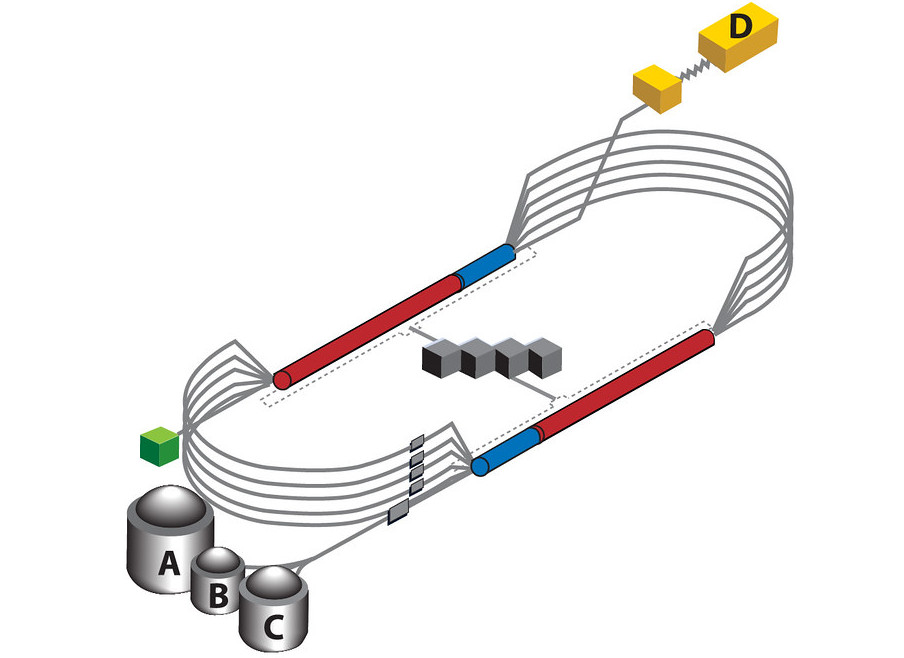
\includegraphics[width=0.5\textwidth]{31cebaf.jpg}}
            }

            \scriptsize{\textit{
                CEBAF diagram.
                The two linear accelerators and experiment halls A to D are pictured.
            }}
        \end{figure}
    \end{center}
\end{frame}

% --+ 10.32 CLAS12 +------------------------------------------------------------
\begin{frame}{CEBAF Large Acceptance Spectrometer for 12 GeV (CLAS12)}
    \label{10.32::clas12}

    \begin{itemize}
        \item
            \ef{CLAS12} is the main particle detector at Hall B.

        \item
            The spectrometer is based on two magnets: a solenoid and a 5 T torus.

        \item
            The CLAS12 Forward Detector (FD) has a \ef{polar coverage from $5\degree$ to $35\degree$} and \ef{full azimuthal coverage}.
    \end{itemize}

    \vspace{-12pt}
    \begin{columns}[onlytextwidth,T]

    \begin{column}{.59\linewidth}
        \begin{center}
            \begin{figure}[t]
                \centering{
                    \fbox{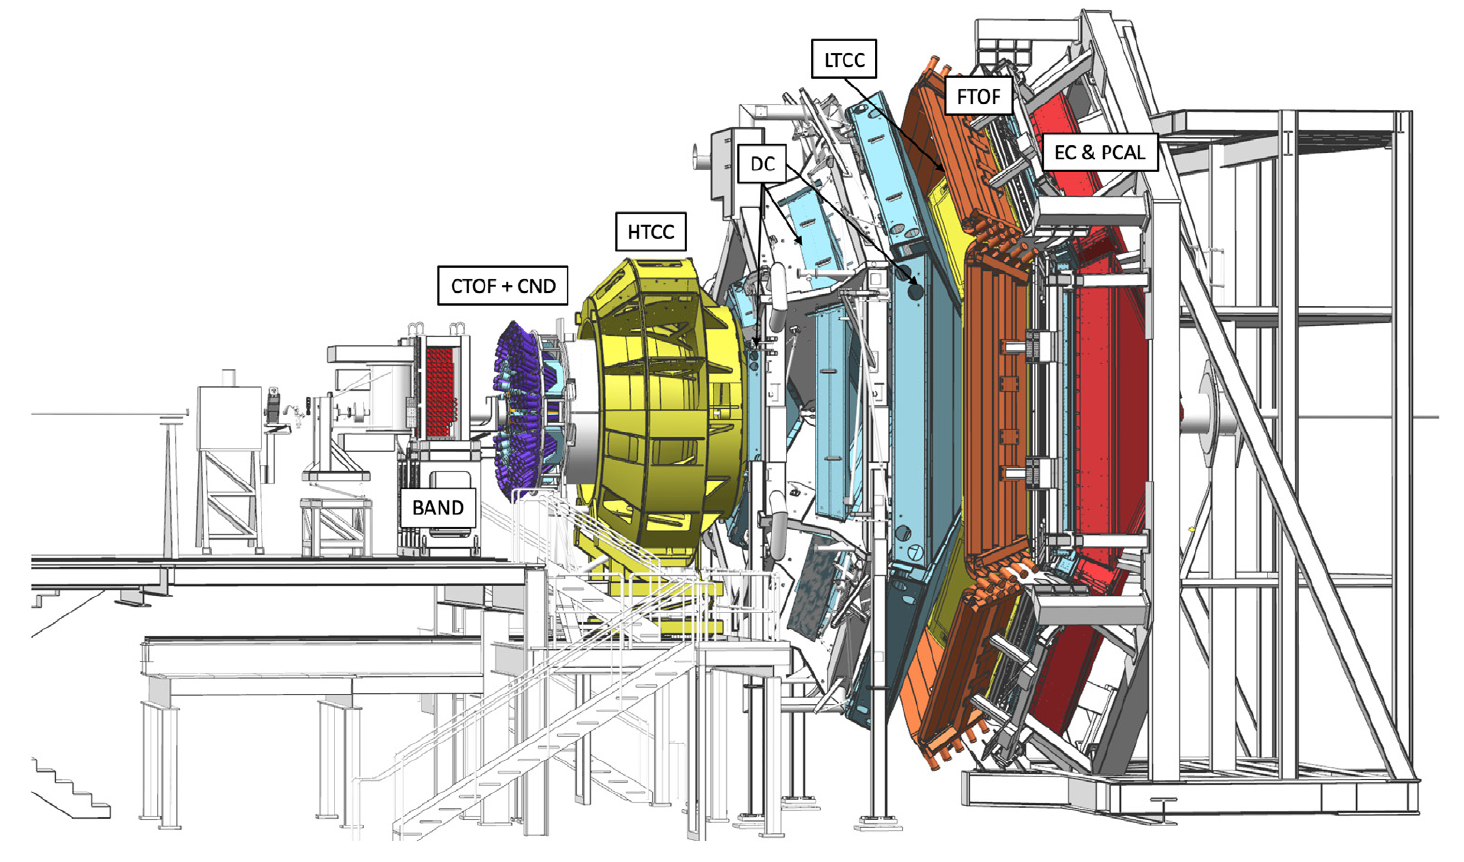
\includegraphics[width=\textwidth]{32clas12.png}}
                }
            \end{figure}
        \end{center}
    \end{column}

    \begin{column}{.39\linewidth}
        \vspace{18pt}
        \small{\textit{
            \ef{CLAS12 diagram.}
            \begin{itemize}
                % \vspace{6pt}
                % \item
                %     \ef{BAND}, \ef{CTOF}, and \ef{CND} are not used in this study.
                \vspace{6pt}
                \item
                    \ef{HTCC}, \ef{LTCC}, and \ef{FTOF} are used in particle identification and event time measurement.
                \vspace{6pt}
                \item
                    \ef{EC} and \ef{PCAL} are the forward calorimeters.
                \vspace{6pt}
                \item
                    \ef{DC} and \ef{FMT} are the forward particle trackers.
            \end{itemize}
        }}
    \end{column}

    \end{columns}
\end{frame}

% --+ 10.33 DC +----------------------------------------------------------------
\begin{frame}{Drift Chambers (DC)}
    \label{10.33::dc}

    \begin{itemize}
        \item
            The DC is the main \ef{tracking detector} of the FD.

        \item
            DC detectors use an array of HV wires to detect \ef{ionising particles}.

        \item
            The tracker has a \ef{momentum resolution of $\Delta p/p < 0.5\%$}, allowing for accurate reconstruction of particle trajectories.
    \end{itemize}

    \vspace{-12pt}
    \begin{columns}[onlytextwidth,T]

    \begin{column}{.44\linewidth}
        \begin{center}
            \begin{figure}[t]
                \centering{
                    \fbox{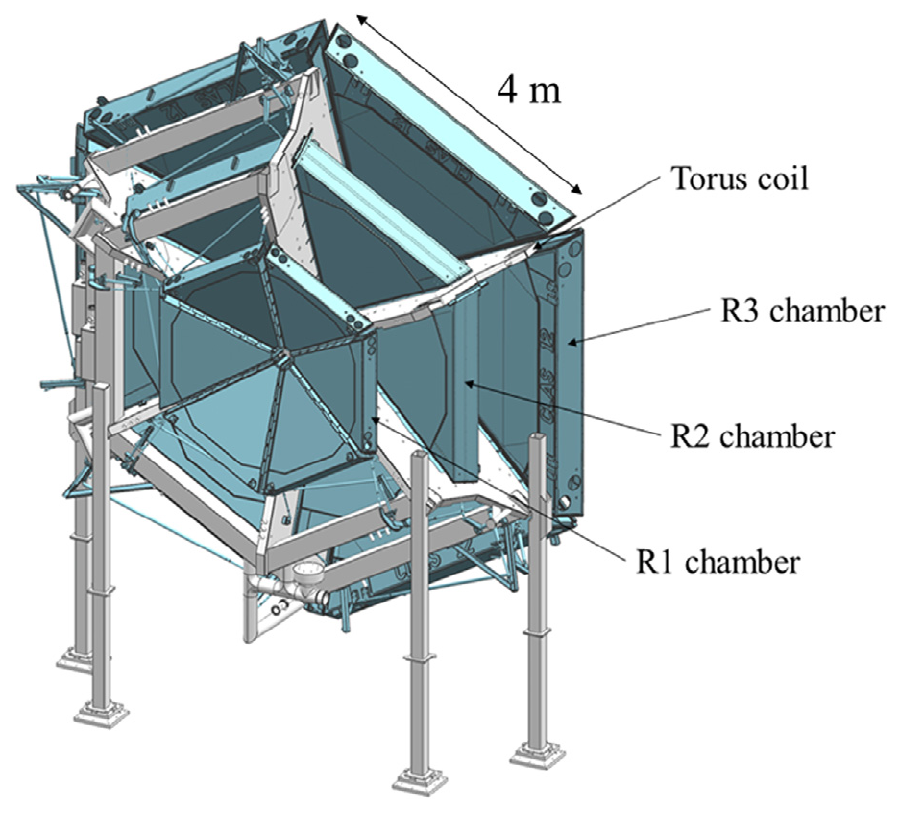
\includegraphics[width=\textwidth]{33dc.png}}
                }
            \end{figure}
        \end{center}
    \end{column}

    \begin{column}{.55\linewidth}
        \vspace{42pt}
        \scriptsize{\textit{
            \ef{3d render of the DC.}
            \begin{itemize}
                \vspace{6pt}
                \item
                    Three independent drift chambers are installed in each of the six sectors of the torus magnet.
                \vspace{6pt}
                \item
                    Each sector contains a total of \ef{36 DC layers}, each with \ef{112 sense wires}.
                \vspace{6pt}
                \item
                    Polar resolution: \ef{$\Delta\theta < 2$} \textcolor{efd_green}{mrad}.
                \vspace{6pt}
                \item
                    azimuthal resolution: \ef{$\Delta\phi < 2$} \textcolor{efd_green}{mrad}.
            \end{itemize}
        }}
    \end{column}

    \end{columns}
\end{frame}

% --+ 10.34 FMT +---------------------------------------------------------------
\begin{frame}{Forward Micromegas Tracker (FMT)}
    \label{10.34::fmt}

    \begin{columns}[onlytextwidth,T]

    \begin{column}{.48\linewidth}
        \vspace{6pt}
        \begin{itemize}
            \item
                FMT is the forwards part of the Micromegas Vertex Tracker (MVT).
                It's first layer sits at \ef{$z \approx 26$} \textcolor{efd_green}{cm}.

            \vspace{6pt}
            \item
                It uses micromegas tracking technology to detect charged particles that cross it\appref{20.07::micromegas_tracking}.

            \vspace{6pt}
            \item
                The detector works in tandem with the DC to do \ef{forward particle tracking}.

            \vspace{6pt}
            \item
                To get an accurate picture of the passing particle, FMT has \ef{3 layers}, each rotated $60\degree$ with respect to the previous one\appref{20.08::fmt_geometry}.

        \end{itemize}
    \end{column}

    \begin{column}{.50\linewidth}
        \begin{center}
            \begin{figure}[t]
                \fbox{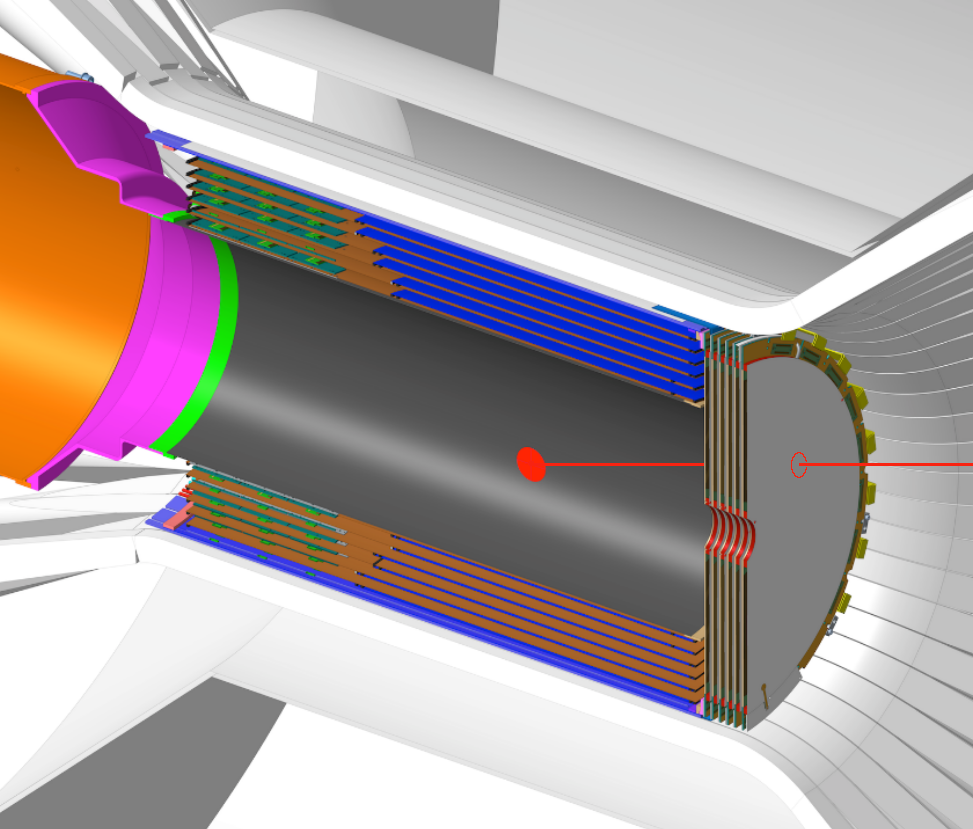
\includegraphics[width=0.95\textwidth]{34mvt_geometry.png}}

                \scriptsize{\textit{
                    \ef{3d render of MVT.}
                    The red dot denotes $z=0$.
                    The red line denote an arbitrary track crossing FMT.
                }}
            \end{figure}
        \end{center}
    \end{column}

    \end{columns}
\end{frame}
